\documentclass{article}\usepackage[]{graphicx}\usepackage[]{color}
% maxwidth is the original width if it is less than linewidth
% otherwise use linewidth (to make sure the graphics do not exceed the margin)
\makeatletter
\def\maxwidth{ %
  \ifdim\Gin@nat@width>\linewidth
    \linewidth
  \else
    \Gin@nat@width
  \fi
}
\makeatother

\definecolor{fgcolor}{rgb}{0.345, 0.345, 0.345}
\newcommand{\hlnum}[1]{\textcolor[rgb]{0.686,0.059,0.569}{#1}}%
\newcommand{\hlstr}[1]{\textcolor[rgb]{0.192,0.494,0.8}{#1}}%
\newcommand{\hlcom}[1]{\textcolor[rgb]{0.678,0.584,0.686}{\textit{#1}}}%
\newcommand{\hlopt}[1]{\textcolor[rgb]{0,0,0}{#1}}%
\newcommand{\hlstd}[1]{\textcolor[rgb]{0.345,0.345,0.345}{#1}}%
\newcommand{\hlkwa}[1]{\textcolor[rgb]{0.161,0.373,0.58}{\textbf{#1}}}%
\newcommand{\hlkwb}[1]{\textcolor[rgb]{0.69,0.353,0.396}{#1}}%
\newcommand{\hlkwc}[1]{\textcolor[rgb]{0.333,0.667,0.333}{#1}}%
\newcommand{\hlkwd}[1]{\textcolor[rgb]{0.737,0.353,0.396}{\textbf{#1}}}%
\let\hlipl\hlkwb

\usepackage{framed}
\makeatletter
\newenvironment{kframe}{%
 \def\at@end@of@kframe{}%
 \ifinner\ifhmode%
  \def\at@end@of@kframe{\end{minipage}}%
  \begin{minipage}{\columnwidth}%
 \fi\fi%
 \def\FrameCommand##1{\hskip\@totalleftmargin \hskip-\fboxsep
 \colorbox{shadecolor}{##1}\hskip-\fboxsep
     % There is no \\@totalrightmargin, so:
     \hskip-\linewidth \hskip-\@totalleftmargin \hskip\columnwidth}%
 \MakeFramed {\advance\hsize-\width
   \@totalleftmargin\z@ \linewidth\hsize
   \@setminipage}}%
 {\par\unskip\endMakeFramed%
 \at@end@of@kframe}
\makeatother

\definecolor{shadecolor}{rgb}{.97, .97, .97}
\definecolor{messagecolor}{rgb}{0, 0, 0}
\definecolor{warningcolor}{rgb}{1, 0, 1}
\definecolor{errorcolor}{rgb}{1, 0, 0}
\newenvironment{knitrout}{}{} % an empty environment to be redefined in TeX

\usepackage{alltt}
\title{A dietary intervention to alleviate flares after treatment reduction for SpA patients in stable low disease activity;\\Preliminary study design and power analysis.}
\author{Koray Taşcılar}

\usepackage{booktabs}
\usepackage{longtable}
\usepackage{array}
\usepackage{multirow}
\usepackage{wrapfig}
\usepackage{float}
\usepackage{colortbl}
\usepackage{pdflscape}
\usepackage{tabu}
\usepackage{threeparttable}
\usepackage{threeparttablex}
\usepackage[normalem]{ulem}
\usepackage[normalem]{ulem}
\usepackage[utf8]{inputenc}
\usepackage{makecell}
\usepackage{xcolor}
\usepackage[margin=2.5cm]{geometry}
\usepackage{appendix}
\usepackage{tikz}
\usepackage{amsmath}
\IfFileExists{upquote.sty}{\usepackage{upquote}}{}
\begin{document}
\maketitle

\begin{knitrout}
\definecolor{shadecolor}{rgb}{0.969, 0.969, 0.969}\color{fgcolor}\begin{kframe}
\begin{alltt}
\hlkwd{library}\hlstd{(tidyverse)}
\end{alltt}
\end{kframe}
\end{knitrout}

\section {Study design}
This is a 6-month interventional study to evaluate the effect of a high fiber dietary supplement that stimulates the production of short chain fatty acids in the gut. The study will include ankylosing spondylitis (AS) patients diagnosed on the basis of New York Criteria (1984) or axial spondyloarthritis (SpA) patients fulfilling the Assessment of SpondyloArthritis international Society (ASAS) 2009 criteria. Included patients will be required to be in stable low disease activity defined as an ASDAS score (Figure \ref{fig:asdas} on page \pageref{fig:asdas}) less than 1.2 in 2 consecutive visits for at least 6 months before inclusion. The ASDAS threshold defines the low disease activity as proposed by the  ASAS (Figure \ref{fig:asdasactivity} on page \pageref{fig:asdasactivity}). At baseline we might need to check whether the patients are already receiving any variant of the specific fiber (if yes in which amount) to be tested in the study and consider excluding them if necessary. Study will include 3 arms, namely;
\begin{enumerate}
  \item Control arm that will continue the pre-study treatment. (Control group)
  \item Intervention arm with 50\% reduction of baseline treatment and a low-fiber supplement. (LoFi group)
  \item Intervention arm with 50\% reduction of baseline treatment and a high-fiber supplement. (HiFi group)
\end{enumerate}
\subsection{Primary endpoint}
Primary outcome will be the ASDAS difference from the control arm at last follow-up.
Patients who experience a flare (ASDAS increase by more than 0.9) in any arm are allowed to undergo a rescue treatment of their primary physician‘s choice, they will be considered as failures and the ASDAS at time of the flare will be carried forward for the final analysis.
Primary endpoint will be the final ASDAS.

\begin{figure}
  \centering
  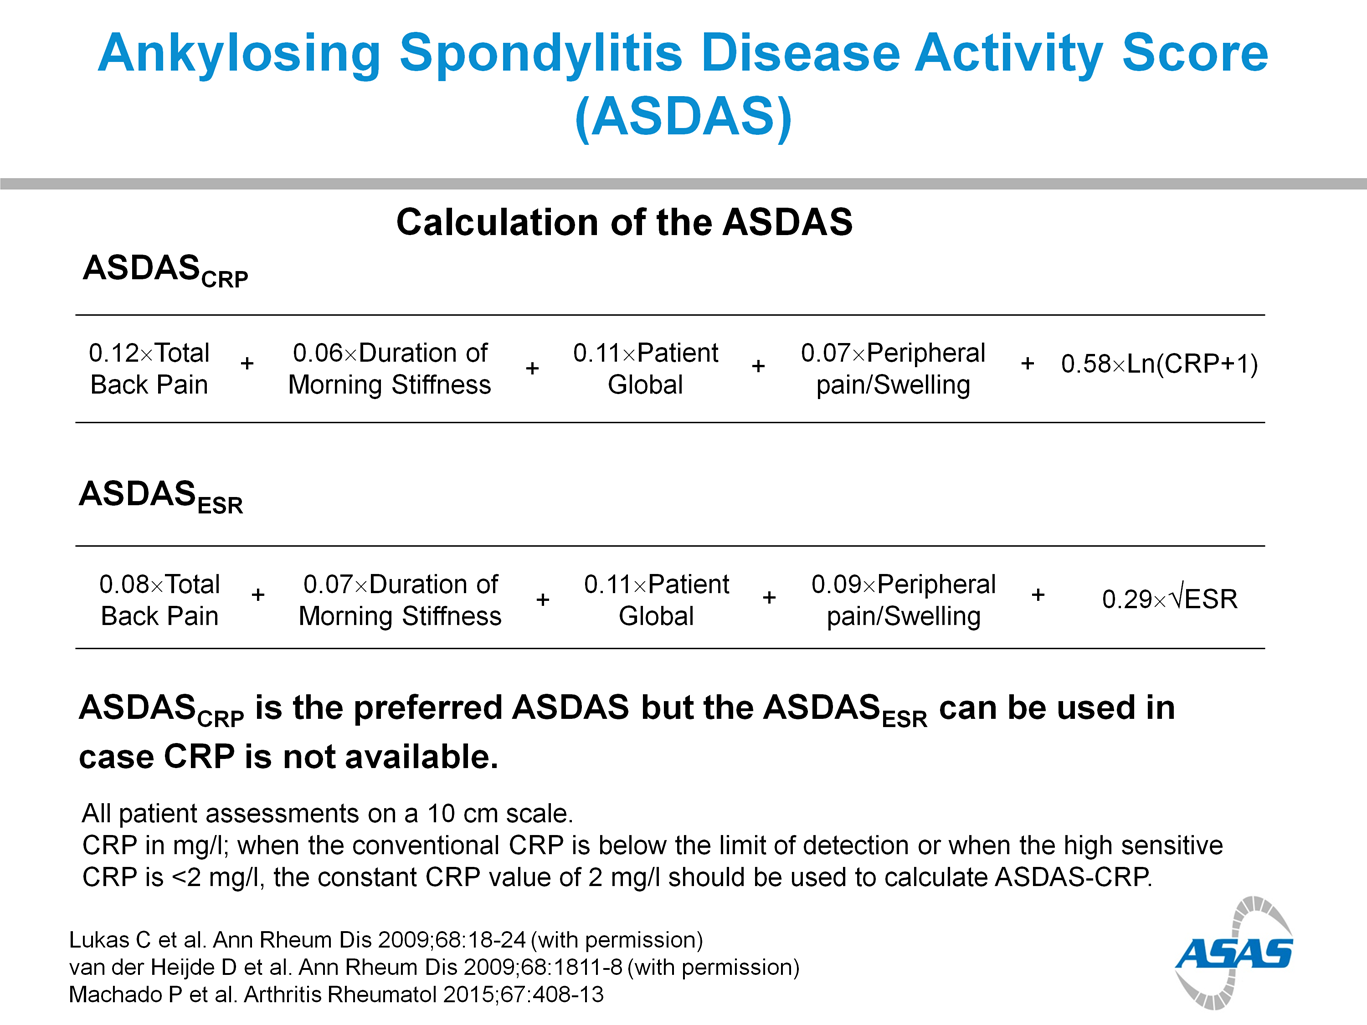
\includegraphics[width=0.75\textwidth]{ASDAS.png}
  \caption {Calculation of ASDAS}
  \label{fig:asdas}
\end{figure}

\begin{figure}
  \centering
  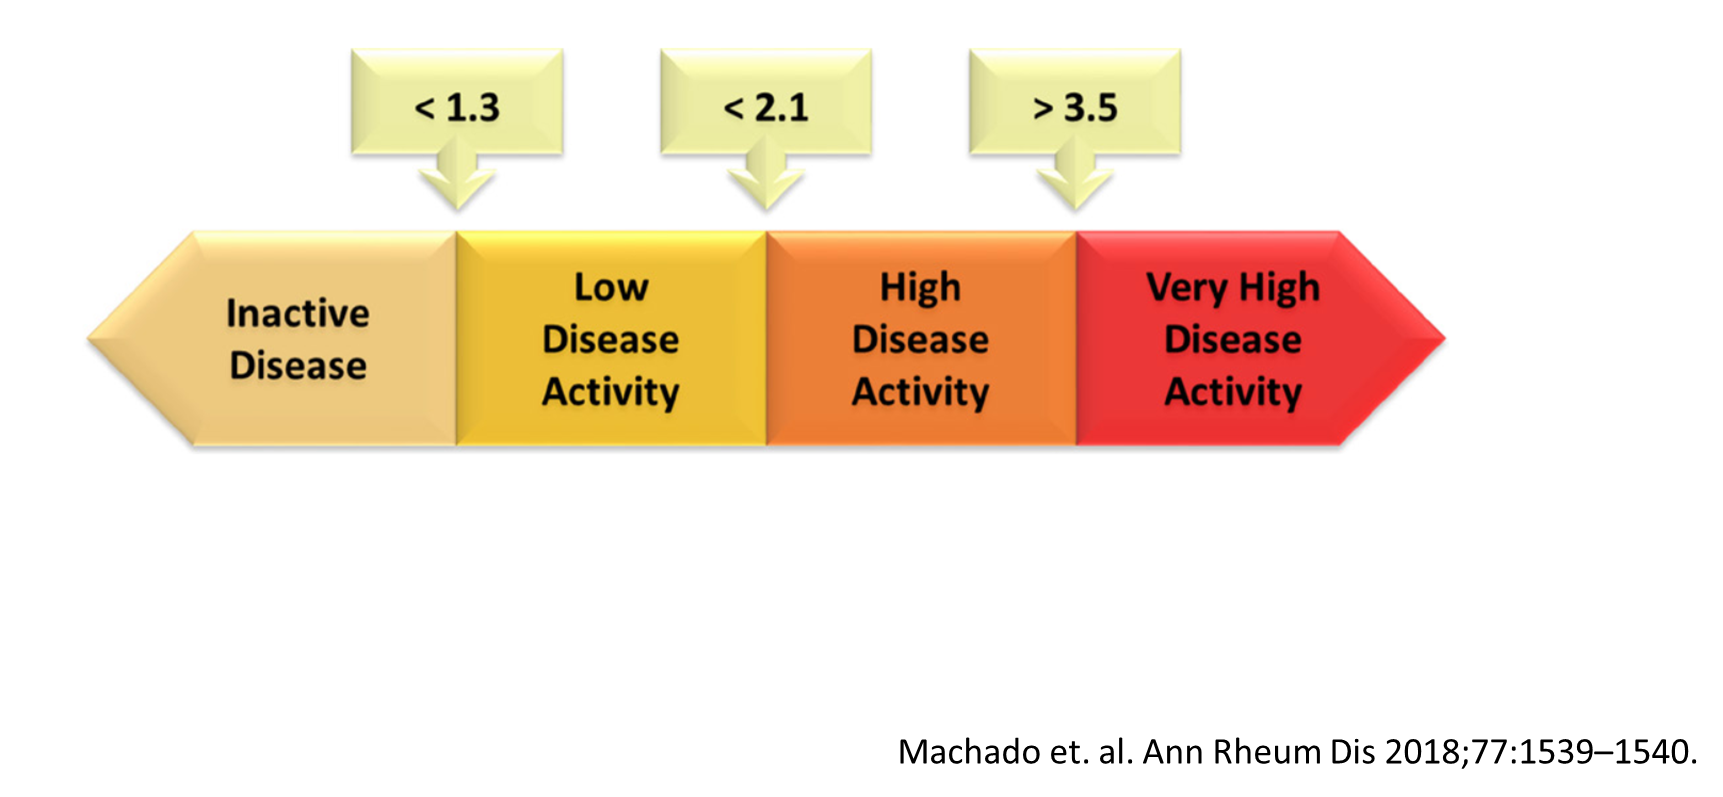
\includegraphics[width=0.75\textwidth]{asdasactivity.png}
  \caption{ASDAS thresholds for disease activity states in SpA}
  \label{fig:asdasactivity}
\end{figure}

\subsection{Primary hypotheses}

\begin{enumerate}
\item HiFi group will be non-inferior to the Control group defined as the single sided 95\%upper confidence limit of  $\overline{ASDAS}_{HiFi} - \overline{ASDAS}_{Control}$ difference that will not exceed the flare definition (0.9)
\item HiFi group will be superior to the LoFi group defined as the point estimate of the mean ASDAS in the HiFi group will be out at the lower side of the ´double sided 95\% confidence interval for the mean final ASDAS in the LoFi group.
\end{enumerate}

\section{Preliminary Power and Sample Size}

Based on these hypotheses, this study will make two co-primary analyses.

\subsection{Non-inferiority outcome}
The first analysis wil include the noninferiority endpoint. Since this trial will include patients in stable remission, we need data from remission studies. In the paper by Lubrano et. al. The mean ASDAS-CRP in an AS population under remission was 1.1 with 25th and 75th percentiles of 0.6 to 1.5. Possible standard deviations that would give these quartile bounds could be as follows assuming normal distribution.
\begin{knitrout}
\definecolor{shadecolor}{rgb}{0.969, 0.969, 0.969}\color{fgcolor}\begin{kframe}
\begin{alltt}
\hlkwd{qnorm}\hlstd{(}\hlkwc{p}\hlstd{=}\hlnum{0.25}\hlstd{,}\hlkwc{mean}\hlstd{=}\hlnum{1.1}\hlstd{,} \hlkwc{sd}\hlstd{=}\hlnum{0.7}\hlstd{)}
\end{alltt}
\begin{verbatim}
## [1] 0.6278572
\end{verbatim}
\begin{alltt}
\hlkwd{qnorm}\hlstd{(}\hlkwc{p}\hlstd{=}\hlnum{0.75}\hlstd{,}\hlkwc{mean}\hlstd{=}\hlnum{1.1}\hlstd{,} \hlkwc{sd}\hlstd{=}\hlnum{0.6}\hlstd{)}
\end{alltt}
\begin{verbatim}
## [1] 1.504694
\end{verbatim}
\end{kframe}
\end{knitrout}

So we could expect the standard deviation in an AS population with a mean ASDAS-CRP of 1.1 to be in the range of 0.6-0.7.
With this assumption if we want to show non-inferiority of the HiFi intervention from the control group The power calculation will be as follows
\begin{knitrout}
\definecolor{shadecolor}{rgb}{0.969, 0.969, 0.969}\color{fgcolor}\begin{kframe}
\begin{alltt}
\hlstd{muA}\hlkwb{=}\hlnum{1.1} \hlcom{#mean in treatment group}
\hlstd{muB}\hlkwb{=}\hlnum{1.1} \hlcom{#mean in control group}
\hlstd{delta}\hlkwb{=}\hlnum{0.9} \hlcom{#non-inferiority margin}
\hlstd{kappa}\hlkwb{=}\hlnum{1} \hlcom{#sampling ratio}
\hlstd{sd}\hlkwb{=}\hlnum{0.8} \hlcom{#standard deviation}
\hlstd{alpha}\hlkwb{=}\hlnum{0.025} \hlcom{#type 1 error}
\hlstd{beta}\hlkwb{=}\hlnum{0.10} \hlcom{#type2 error}
\hlstd{(nB}\hlkwb{=}\hlstd{(}\hlnum{1}\hlopt{+}\hlnum{1}\hlopt{/}\hlstd{kappa)}\hlopt{*}\hlstd{(sd}\hlopt{*}\hlstd{(}\hlkwd{qnorm}\hlstd{(}\hlnum{1}\hlopt{-}\hlstd{alpha)}\hlopt{+}\hlkwd{qnorm}\hlstd{(}\hlnum{1}\hlopt{-}\hlstd{beta))}\hlopt{/}\hlstd{(muA}\hlopt{-}\hlstd{muB}\hlopt{-}\hlstd{delta))}\hlopt{^}\hlnum{2}\hlstd{)}
\end{alltt}
\begin{verbatim}
## [1] 16.60432
\end{verbatim}
\begin{alltt}
\hlkwd{ceiling}\hlstd{(nB)} \hlcom{# round to the nearest integer}
\end{alltt}
\begin{verbatim}
## [1] 17
\end{verbatim}
\begin{alltt}
\hlstd{z}\hlkwb{=}\hlstd{(muA}\hlopt{-}\hlstd{muB}\hlopt{-}\hlstd{delta)}\hlopt{/}\hlstd{(sd}\hlopt{*}\hlkwd{sqrt}\hlstd{((}\hlnum{1}\hlopt{+}\hlnum{1}\hlopt{/}\hlstd{kappa)}\hlopt{/}\hlstd{nB))}
\hlstd{(Power}\hlkwb{=}\hlkwd{pnorm}\hlstd{(z}\hlopt{-}\hlkwd{qnorm}\hlstd{(}\hlnum{1}\hlopt{-}\hlstd{alpha))}\hlopt{+}\hlkwd{pnorm}\hlstd{(}\hlopt{-}\hlstd{z}\hlopt{-}\hlkwd{qnorm}\hlstd{(}\hlnum{1}\hlopt{-}\hlstd{alpha)))}
\end{alltt}
\begin{verbatim}
## [1] 0.9000001
\end{verbatim}
\end{kframe}
\end{knitrout}

So this means if we define noninferiority as the 97.5 \% one sided upper confidence limit of ASDAS difference not exceeding 0.9, we need to include at least 17 patients per arm for 90\% power and a one sided alpha error rate of 0.025 (Chow S, Shao J, Wang H. 2008. Sample Size Calculations in Clinical Research. 2nd Ed. Chapman & Hall/CRC Biostatistics Series.). We assumed a pessimistic scenario and that the standard deviation would be higher than observed. If we assume a 25\% droup out rate the per group sample size should be at least 23 per group for the non-inferiority study.

\subsection{Superiority outcome}

The second hypothesis in this study is that the final ASDAS in the HiFi group will be better than that in the LoFi group. In order to detect a mean difference of 0.9 between groups assuming a standard deviation of 0.9 and a control group mean ASDAS of 1.1 with 90\%power and a two sided alpha error rate of 0.025 the required sample size would be calculated as follows.
\begin{knitrout}
\definecolor{shadecolor}{rgb}{0.969, 0.969, 0.969}\color{fgcolor}\begin{kframe}
\begin{alltt}
\hlstd{muA}\hlkwb{=}\hlnum{1.1} \hlcom{#Expected mean ASDAS at study end in the HiFi group}
\hlstd{muB}\hlkwb{=}\hlnum{2.0} \hlcom{#Expected mean ASDAS at study end in the LoFi group}
\hlstd{kappa}\hlkwb{=}\hlnum{1} \hlcom{#Enrollment ratio 1:1}
\hlstd{sd}\hlkwb{=}\hlnum{0.9} \hlcom{# Expected standard deviation}
\hlstd{alpha}\hlkwb{=}\hlnum{0.025} \hlcom{#Two sided alpha error rate}
\hlstd{beta}\hlkwb{=}\hlnum{0.10} \hlcom{#Beta error rate}
\hlstd{(nB}\hlkwb{=}\hlstd{(}\hlnum{1}\hlopt{+}\hlnum{1}\hlopt{/}\hlstd{kappa)}\hlopt{*}\hlstd{(sd}\hlopt{*}\hlstd{(}\hlkwd{qnorm}\hlstd{(}\hlnum{1}\hlopt{-}\hlstd{alpha}\hlopt{/}\hlnum{2}\hlstd{)}\hlopt{+}\hlkwd{qnorm}\hlstd{(}\hlnum{1}\hlopt{-}\hlstd{beta))}\hlopt{/}\hlstd{(muA}\hlopt{-}\hlstd{muB))}\hlopt{^}\hlnum{2}\hlstd{)}
\end{alltt}
\begin{verbatim}
## [1] 24.82241
\end{verbatim}
\begin{alltt}
\hlkwd{ceiling}\hlstd{(nB)} \hlcom{# round to the nearest integer}
\end{alltt}
\begin{verbatim}
## [1] 25
\end{verbatim}
\begin{alltt}
\hlstd{z}\hlkwb{=}\hlstd{(muA}\hlopt{-}\hlstd{muB)}\hlopt{/}\hlstd{(sd}\hlopt{*}\hlkwd{sqrt}\hlstd{((}\hlnum{1}\hlopt{+}\hlnum{1}\hlopt{/}\hlstd{kappa)}\hlopt{/}\hlstd{nB))}
\hlstd{(Power}\hlkwb{=}\hlkwd{pnorm}\hlstd{(z}\hlopt{-}\hlkwd{qnorm}\hlstd{(}\hlnum{1}\hlopt{-}\hlstd{alpha}\hlopt{/}\hlnum{2}\hlstd{))}\hlopt{+}\hlkwd{pnorm}\hlstd{(}\hlopt{-}\hlstd{z}\hlopt{-}\hlkwd{qnorm}\hlstd{(}\hlnum{1}\hlopt{-}\hlstd{alpha}\hlopt{/}\hlnum{2}\hlstd{)))}
\end{alltt}
\begin{verbatim}
## [1] 0.9
\end{verbatim}
\end{kframe}
\end{knitrout}

Meaning that for the superiority comparison we need at least 25 patients per each arm. Again allowing a dropout rate of 25\% the number of patients to be enrolled would be at least 34 per arm.

With a one to one randomization ratio for each arm we could estimate the total number as thrice the highest estimated sample size and that makes 112 participants to be randomized to three study arms. Overall study outline is depicted in Figure \ref{fig:studyoutline} on page \pageref{fig:studyoutline}

\begin{figure}
  \centering
  \frame{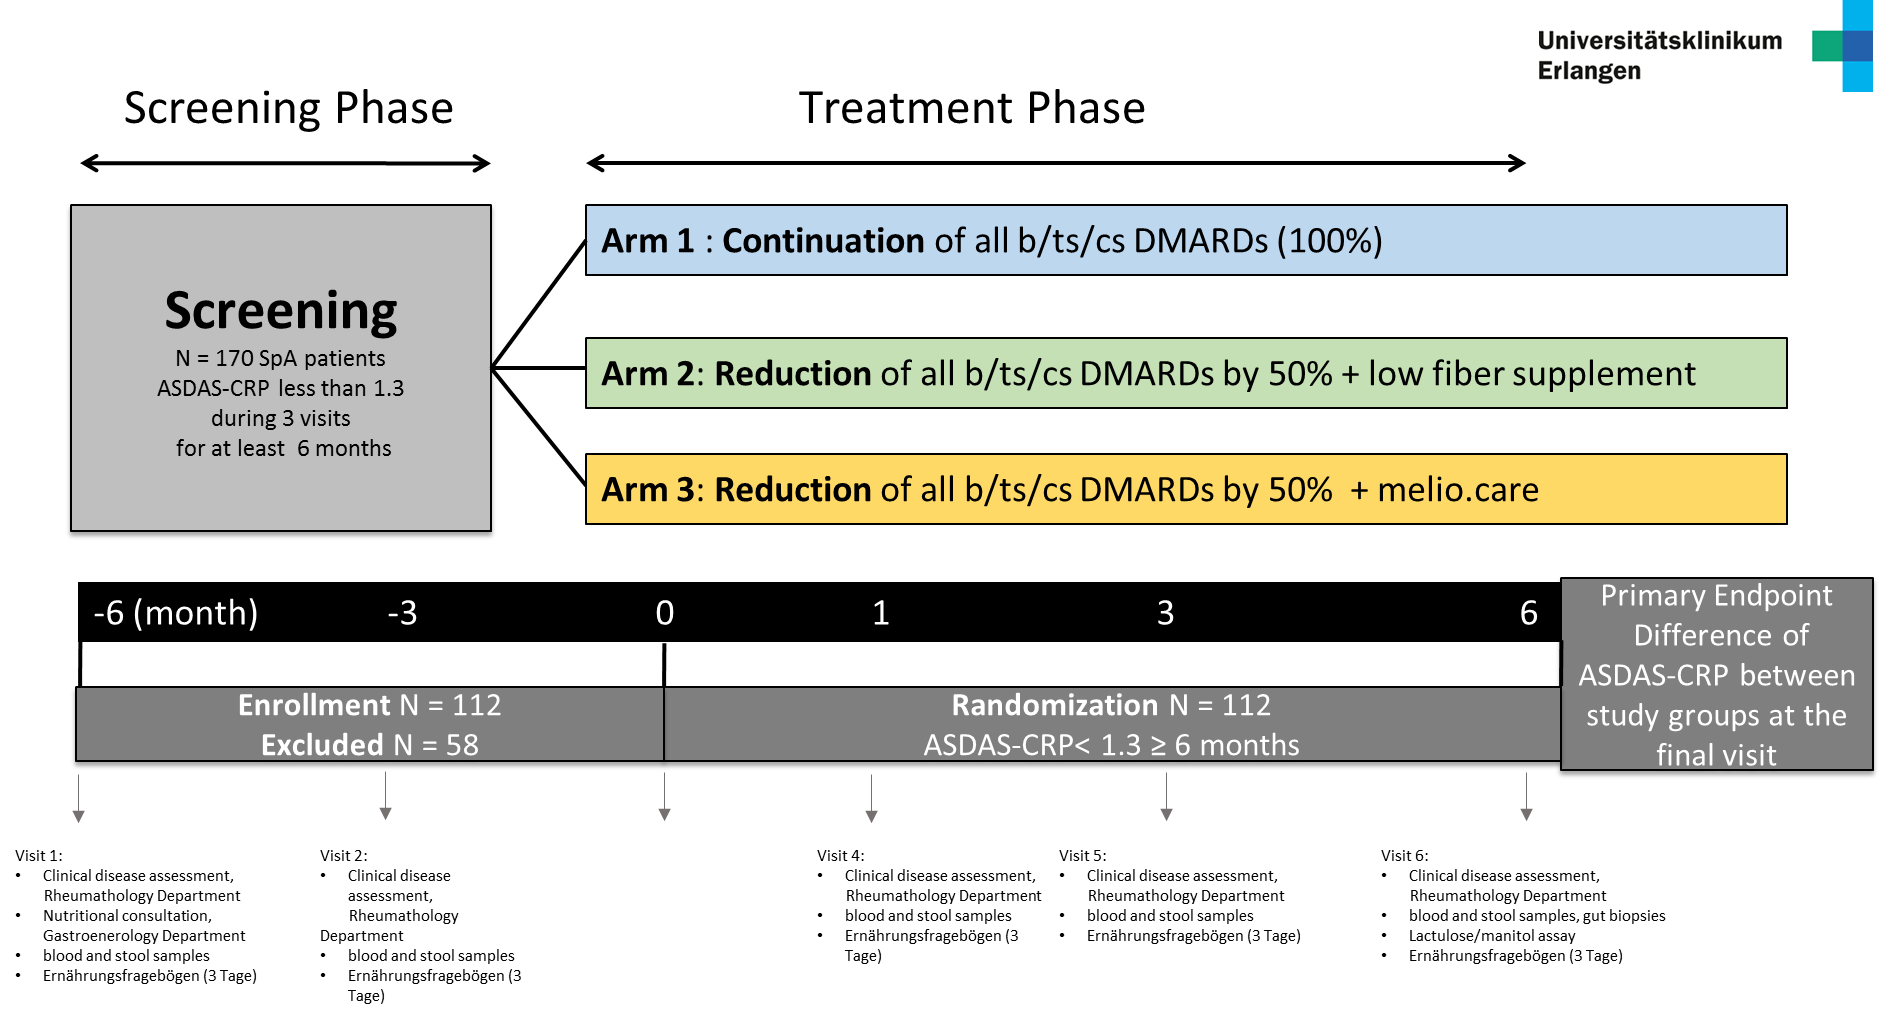
\includegraphics[width=1\textwidth]{studyoutline.png}}
  \caption {Summary of study design and study procedures.}
  \label{fig:studyoutline}
\end{figure}
\end{document}
